\chapter{Conceptual Model}

Figure~\ref{fig:con-model} shows an example of the main page for user interface. This page shows what the interaction page should look like when the user is playing the game. There are three options provided for the users that they can click on. The baby will react differently to different options.

\begin{figure}[H]
    \centering
    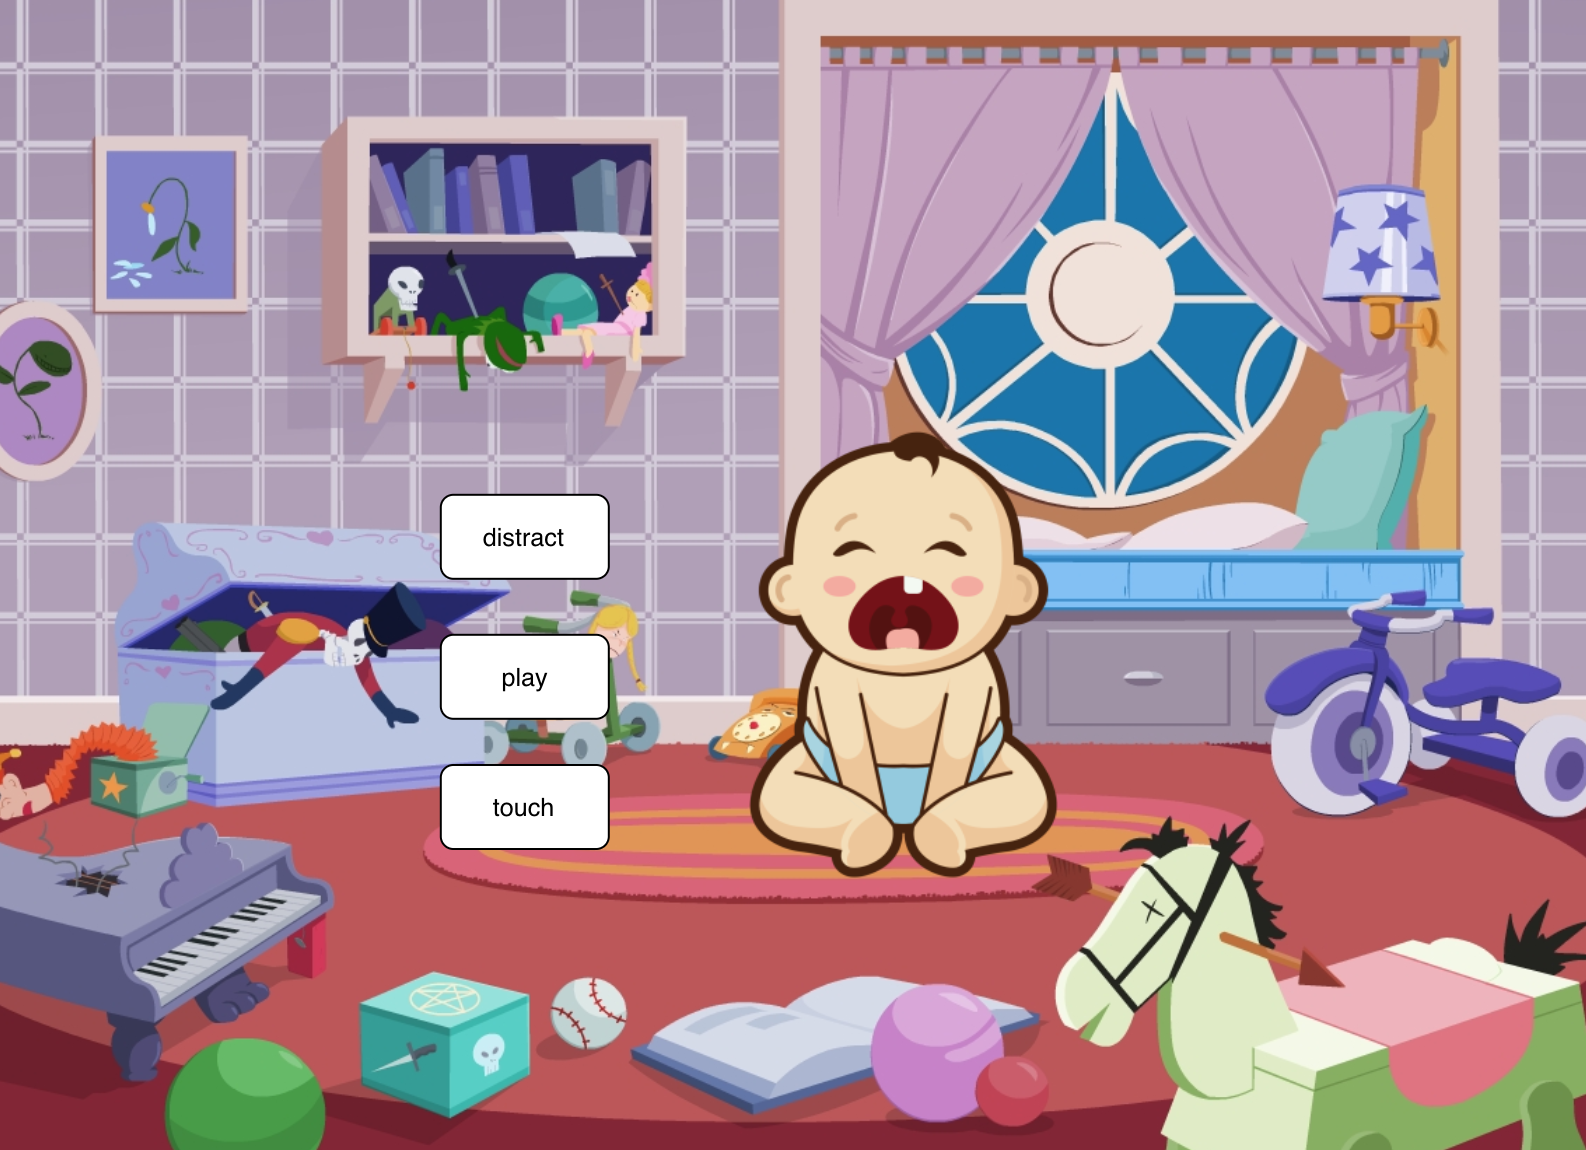
\includegraphics[width=0.75\linewidth]{conceptual-model.png}
    \caption{Conceptual Model}
    \label{fig:con-model}
\end{figure}
The users can access both the report on a single practice, and the general progress report which shows all of their practice. 

Figure~\ref{fig:report} is an example of the report that the user can view. In the report on a specific practice, the users can see the time they first got stressed and the level of stress they experienced. 

\begin{figure}[H]
    \centering
    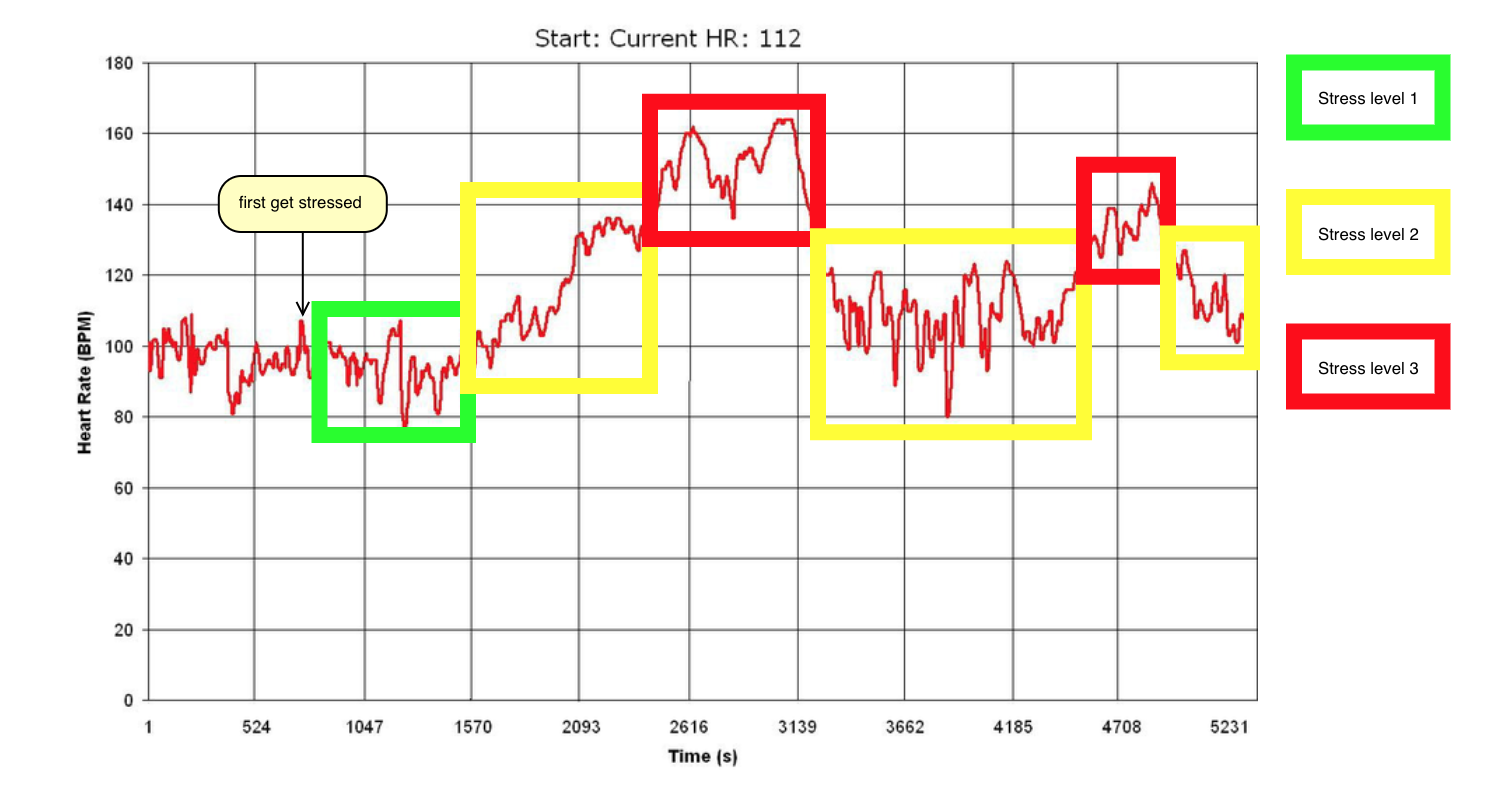
\includegraphics[width=0.75\linewidth]{heartrate.png}
    \caption{Report}
    \label{fig:report}
\end{figure}

Figure~\ref{fig:prog-rep} is an example of the progress report that the user can view. In the progress report, the users can compare their performance in different practices and check their progress under the same difficulty level.

\begin{figure}[H]
    \centering
    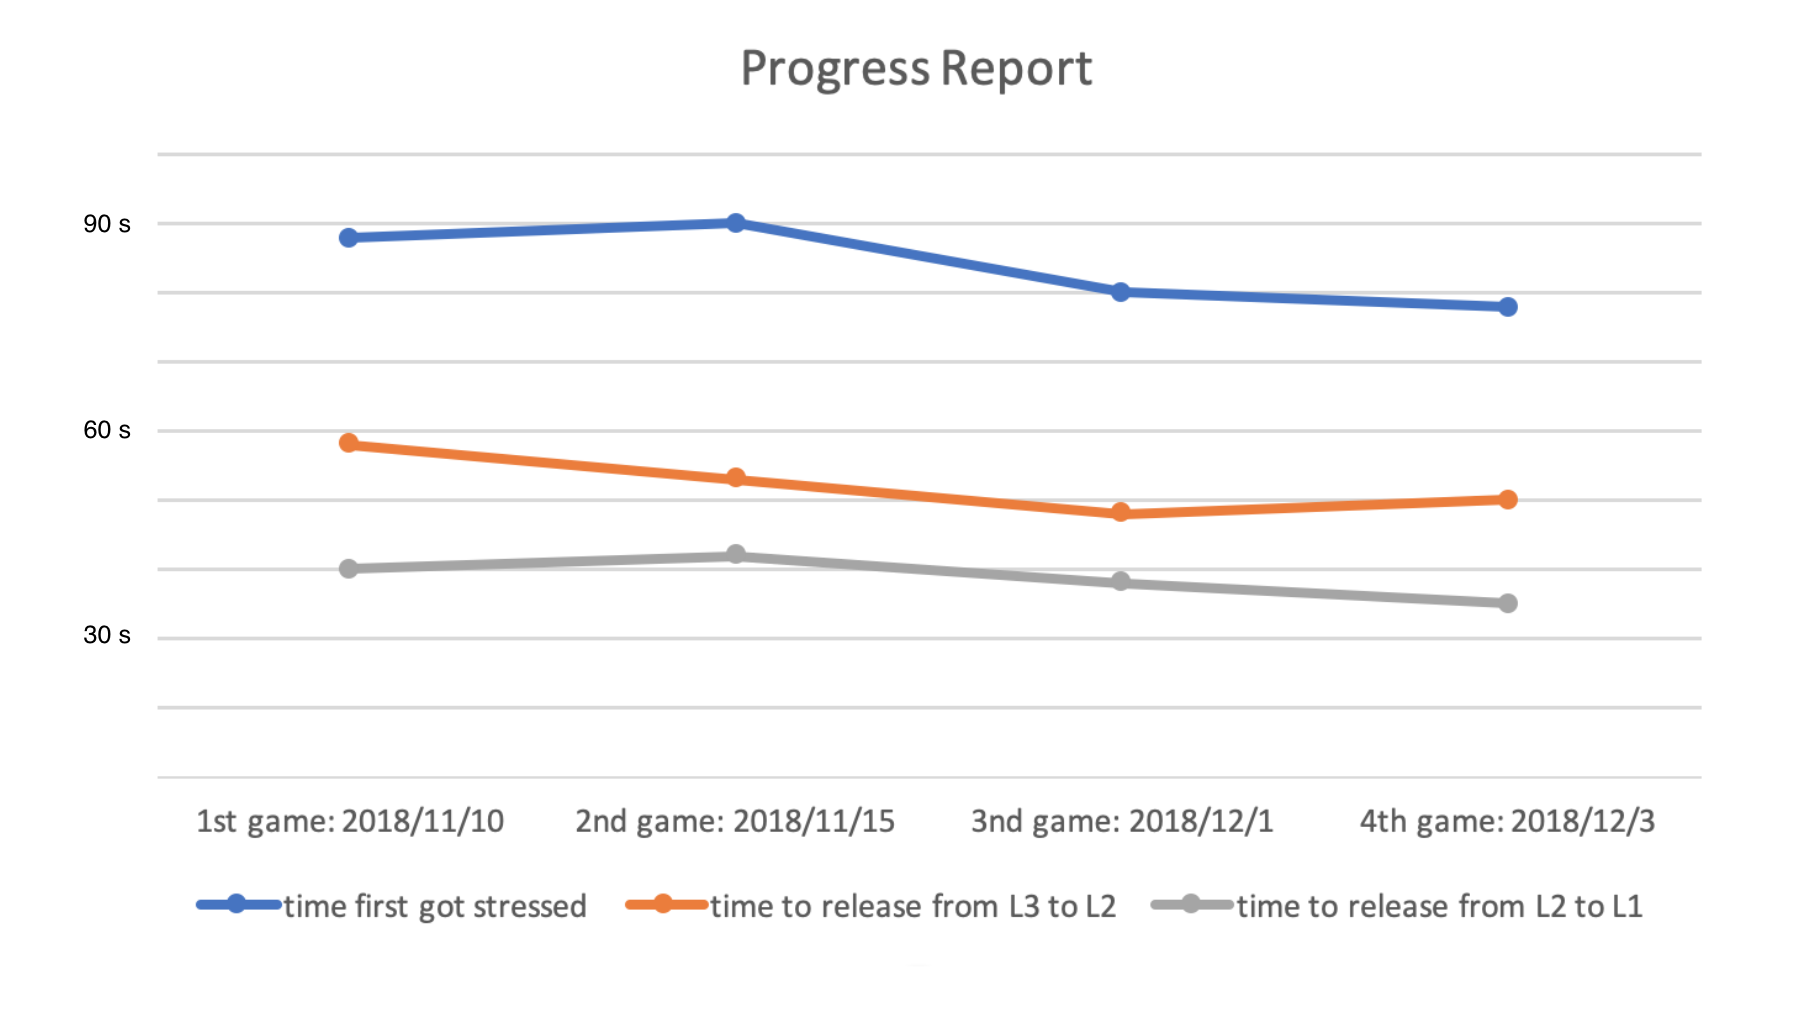
\includegraphics[width=0.75\linewidth]{progress-report.png}
    \caption{Progress Report}
    \label{fig:prog-rep}
\end{figure} 










